\chapter{Espace topologique}

La topologie constitue l’un des fondements essentiels des mathématiques, car elle permet d’étudier les notions de continuité, de voisinage et de convergence dans un cadre général. Dans ce chapitre, nous allons approfondir les concepts d’espaces topologiques, d’ouverts et de fermés, ainsi que les propriétés fondamentales liées aux suites et aux applications continues. L’objectif est de développer une compréhension rigoureuse des structures topologiques afin de mieux saisir les liens entre analyse, géométrie et autres branches des mathématiques.

\section{Constructions de topologies}
 
Dans cette section, nous allons considérer plusieurs façons d'associer à un ensemble ce qu'on appelle un espace topologique.
\subsection{Filtres et voisinages}
\begin{definition}
    Soit $X\ne \varnothing$. Soit $\filtre\subseteq\partie(X)$ non vide. $\filtre$ est un filtre sur $X$ si $\filtre$ vérifie les propriétés suivantes
    
    \begin{enumerate}
        \item $\varnothing\notin\filtre$
        \item $\forall A,B\in \filtre \quad A\cap B\in \filtre$
        \item $\forall A\in \filtre,\forall B\in \partie(X) \quad (A\subseteq B)\Rightarrow(B\in \filtre)$
    \end{enumerate}
    
\end{definition}

\begin{remarque}
    Dans un filtre $\filtre$, on a toujours $X\in \filtre$. En effet, $\filtre\neq\varnothing$ on en déduit donc  l'existence d'un $A\in \filtre$, d'où $X\in\filtre$ car $A\subseteq X\in\partie(X)$.
\end{remarque}
\begin{notation}
    Soit $\varnothing\ne Y\subseteq X$. On note par $\filtre_Y := \{ Z\in\partie X\mid Y\subseteq Z\}$ le filtre engendré par $Y$. Il s'agit d'un filtre sur $X$
\end{notation}
\begin{proof} Montrons que $\filtre_Y$ satisfait les axiomes des filtres.
    \begin{enumerate} 
        \item Soit $A\in\filtre_Y$. Clairement, $A\ne \varnothing$, car sinon, on aurait $Y\subseteq \varnothing$ d'où $Y = \varnothing$.
        \item Clairement, si $Y\subseteq A$ et $B\subseteq X$, alors on a $Y\subseteq A \cap B\subseteq X$.
        \item Si $Y\subseteq A\subseteq X$ et $B\subseteq X$, alors on a par transitivité, $Y\subseteq B\subseteq X$.
    \end{enumerate}
\end{proof}
\begin{notation}
    Lorsque le contexte est clair (par exemple si il est certain que $\forall a\in X,\ \neg(a\subseteq X)$), on simplifie l'écriture de $\filtre_{\{a\}}$ en notant $\filtre_a$. 
\end{notation}
\begin{proposition}
Si $\mathscr{G}$ est un filtre étendant $\filtre_a$ \textit{i.e} $\mathscr G$ est un filtre tel que $\filtre_a \subseteq\mathscr{G}$ alors $\mathscr{G}=\filtre_a$.  On dit que $\filtre_a$ est un ultrafiltre.
\end{proposition}
\begin{proof}
En effet, soit $B\in \mathscr{G}$. Supposons par l'absurde que $a\notin B$. 
Alors $\{a\}\cap B = \varnothing$. 
Or $\{a\}\in\mathscr{G}$ et $B\in\mathscr{G}$, donc par stabilité des filtres par intersection finie, 
on aurait $\varnothing \in \mathscr{G}$, ce qui est absurde. 
Ainsi $a\in B$, donc $B\in \filtre_a$. 
On conclut que $\mathscr{G}\subseteq \filtre_a$.
\end{proof}

\begin{exemple}[Filtre de Frêchet]On appelle filtre de Frêchet, ou filtre des cofinis de $X$, le filtre $\{A\subseteq X \mid X\setminus A \text{ est fini}\}$
\end{exemple}

\begin{proposition}
    Soit $X\ne\varnothing$ un ensemble fini. Alors, l'ensemble des filtres sur $X$ est $\{\filtre_Y\mid Y\subseteq X\}$ 
\end{proposition}
\begin{proof}
    Clairement, les $\filtre_Y$ sont des filtres sur $X$. Réciproquement, soit $\filtre$ un filtre sur $X$. Alors, par définition des filtres, $Y:=\bigcap_{A\in\filtre}A\in\filtre$ car $\filtre\subseteq\partie(X)$ est fini. En effet, $X$ est fini, donc $\partie(X)$ l'est aussi. 
\end{proof}

\begin{definition}
    Soit $X\neq \varnothing$. On dit que $\voisinage:=\left(\voisinage_a\right)_{a\in X}$ est une famille (d'ensemble) de voisinages de points de $X$ si les propriétés suivantes sont vérifiées.    
    \begin{enumerate}
        \item $\forall a\in X, \voisinage_a$ est un filtre sur $X$
        \item $\forall a \in X,\forall V\in\voisinage_a, a\in V $
        \item  $\forall a\in X,\forall V\in \voisinage_a\text{ alors }\exists W\in \voisinage_a\quad W\subseteq V$ et $\forall w\in W,\; V\in \voisinage_w$ (cohérence)
    \end{enumerate}
\end{definition}
\begin{notation}
    Soient $a\in X, V\subseteq X,\voisinage$ une famille (d'ensembles) de voisinages. On dit que $V$ est un voisinage de $a$ si $V\in\voisinage_a$
\end{notation}
\begin{proposition}
De façon équivalente, on peut remplacer la cohérence par :
$$\forall a\in X,\forall V\in \voisinage_a, \exists W\in \voisinage_a , W\subseteq V, \forall w\in W, W\in \voisinage_w$$  
\end{proposition}
\begin{proof}
    Montrons l'équivalence :
    \begin{description}
    \item[($\si$) : ]Par extension, $W\in\voisinage_w$ implique $V\in\voisinage_w$.
        \item[($\alors$) : ]Soient $a\in X,V\in\voisinage_a$. Prenons $W'=\{x\in V\mid V\in\voisinage_x\}$. Remarquons qu'on a bien $W'\subseteq V$. Soit $x\in W'$. Par définition $V\in\voisinage_x$, on peut donc utiliser $3$ pour obtenir $W_y\in\voisinage_y$ tel que $W\subseteq V$ et $\forall w\in W_y,V\in \voisinage_y$ \textit{i.e.} $W_y\in\voisinage_y$ et $W_y\subseteq W'$. Donc $\forall y\in W',W'\in\voisinage_y$. En particulier, on a $W'\in\voisinage_a$ car $a\in W'$.
    \end{description}
\end{proof}
\begin{definition}
Un espace topologique est la donnée d'un ensemble $X$ non vide et d'une famille de voisinages $\voisinage$ sur $X$.
\end{definition}

\begin{definition}
On définit les deux concepts suivants :
\begin{itemize}
    \item Un ouvert de $(X,\voisinage)$ est un ensemble qui est un voisinage de tous ses points.
    \item Un fermé de $(X,\voisinage)$ est un ensemble dont le complémentaire est un ouvert.
\end{itemize}
\end{definition}

\begin{exemple}[Topologie discrète]
    Pour chaque $a \in X$, prenons $\voisinage_a=\filtre_a$. Montrons que ce choix du filtre $\filtre_a$ pour chaque point $a\in X$ vérifie l'axiome de cohérence.
\end{exemple}
\begin{proof}
    Soit $V\in \voisinage_a$, il faut trouver $W\in \voisinage_a$, $W\subseteq V$ tel que $V$ soit un voisinage de tous les points de $W$. On prend $W=\{a\}$ car $\{a\}\subseteq V$ et $\{a\}$ appartiennent à $\voisinage_a$. On peut aussi prendre $W=V$ car tous les voisinages sont ouverts pour la topologie discrète. On a que l'ensemble des ouverts pour la topologie discrète est $\partie(X)$.
\end{proof}
\subsection{Ouverts}

Les ouverts construits précédemment par la topologie engendré par les voisinages safistont les propriétés suivantes. Comme nous allons le voir nous pouvons  définir cette topologie uniquement grâce à ces propriétés.

\begin{definition}
    Soit $\topologie\subseteq \partie(X)$. On dit que $\topologie$ est une famille d'ouverts de $X$ ssi
    \begin{enumerate}
        \item $\varnothing,X\in \topologie$
        \item Si $(\ouvert_i)_{i\in I}$ est une famille d'éléments de $\topologie$ alors $\bigcup_{i\in I}\ouvert_i\in \topologie$
        \item Si $\ouvert_1$ et $\ouvert_2\in \topologie$, alors $\ouvert_1\cap \ouvert_2\in \topologie$ 
    \end{enumerate}
    Dans ce cas, on dira que $\topologie$ est une topologie.
\end{definition}
\begin{definition}
On définit l'application $$\fonction{\operatorname{int}}{\partie(X)\to \partie(X)}{A\mapsto\bigcup_{\ouvert\in\topologie, \ouvert\subseteq A}\ouvert}$$ L'ensemble $\operatorname{int}(A)$, parfois noté $A^\circ$, est appelé intérieur de $A$. Il s'agit du plus grand ouvert contenu dans $A$.
\end{definition}
\begin{proposition}
    Une intersection quelconque de topologies est une topologie.
\end{proposition}
\begin{proof}
Soit $(\topologie_i)_{i\in I}$ une famille de topologies. Montrons que $\bigcap_{i\in I}\topologie_i$ est une topologie. Vérifions que les trois axiomes sont respectés.
\begin{enumerate}
    \item Comme pour tout $i\in I\quad \topologie_i$ est une topologie, on a $\varnothing, X\in \topologie_i$. Donc on a bien \[\varnothing,X\in \bigcap_{i\in I}\topologie_i\]
    \item Soit $(\ouvert_j)_{j\in J}$ une famille d'éléments de $\bigcap_{i\in I}\topologie_i$ alors montrons que
    \[\bigcup_{j\in J}\ouvert_j\in \bigcap_{i\in I}\topologie_i
    \]
    Cette appartenance est vraie puisque pour tout $j\in J \; \ouvert_j\in \bigcap_{i\in I}\topologie_i$ donc l'union appartient également à $\bigcap_{i\in I}\topologie_i$ car les $\topologie_i$ sont des topologies.
    \item Soit $\ouvert_1,\ouvert_2\in \bigcap_{i\in I}\topologie_i$, montrons que $\ouvert_1\cap\ouvert_2\in \bigcap_{i\in I}\topologie_i$. De même que au point 2), puisque $\ouvert_1$ et $\ouvert_2$ appartiennent tous deux à chacune des topologies $\topologie_i$, leur intersection appartiennent donc également à chacune des topologies et donc $\ouvert_1\cap\ouvert_2$ appartient bien à l'intersections des $\topologie_i$.
\end{enumerate}
\end{proof}
\begin{definition}
    On définit les deux applications suivantes:
    \begin{align*}
        \fonction{\mathscr{V}}{\{\text{ Topologie sur }X\}\to \{ \text{ Famille de voisinage sur } X\}}{ \topologie\mapsto (\voisinage_a)_{a\in X}\text{ avec }\voisinage_a := \{V\subseteq X\mid \exists \ouvert\in \topologie, a\in \ouvert\subseteq V\}}
    \end{align*}
    \begin{align*}
        \fonction{\mathscr{T}}{\{ \text{ Famille de voisinage sur } X\}\to\{\text{ Topologie sur }X\} }{ \voisinage\mapsto \{ \varnothing\}\cup\{V\in\partie(X)\mid \forall x\in\ouvert,\ \ouvert\in\voisinage_x\}}
    \end{align*}   
\end{definition}
Montrons que nos applications sont bien définies, càd que l'image de ces fonctions est bien incluse à leur ensemble d'arrivée respectif.
\begin{proof}
Montrons que nos applications sont bien définies :
    \begin{description}
        \item[Bonne définition de $\mathscr{V}$ :] 
        Soit $\topologie$ une topologie sur $X$. Montrons que $\{(\voisinage_a)_{a\in X}\mid \voisinage_a := \{V\subseteq X\mid \exists \ouvert\in \topologie, a\in \ouvert\subseteq V\}\}$ est une famille de voisinages. Commençons par montrer que $\forall a, \voisinage_a$ est un filtre. Vérifions chaque axiome des filtres :\begin{enumerate}
            \item D'abord, on a $\forall V\in\voisinage_a, a\in V$ par définition, d'où $\varnothing\not\in\voisinage_a$. 
            \item Soient $V_1,V_2\in\voisinage_a$. On veut montrer que $V_1\cap V_2\in\voisinage_a$. Par définition, il existe $\ouvert_1,\ouvert_2\in\topologie$ tels que $a\in\ouvert_1\subseteq V_1,a\in \ouvert_2\subseteq V_2$. On a alors $a\in\ouvert_1\cap\ouvert_2,\ouvert_1\cap\ouvert_2\in\topologie$ et $\ouvert_1\cap\ouvert_2\subseteq V_1\cap V_2$. Il vient $V_1\cap V_2\in\voisinage_a$.
            \item Montrons que $\voisinage_a$ est stable par extension. Soient $V\in\voisinage_a,W\in\partie(X)$. Supposons que $V\subseteq W$. Il vient l'existence de $\ouvert\in\topologie$ tel que $a\in\ouvert\subseteq V\subseteq W$, d'où $W\in\voisinage_a$.
        \end{enumerate}
        On a bien $\forall V\in\voisinage_a, a\in V$ par définition. Il reste à montrer la cohérence. Soit $V\in\voisinage_a$. Soit $\ouvert\in\topologie$ tel que $\ouvert \subseteq V$. Prenons $W=\ouvert$. Soit $w\in W$. On a bien $V\in\voisinage_w$ car $w\in W\subseteq V$.
        \item[Bonne définition de $\mathscr{T}$] Soit $\voisinage$ une famille de voisinages sur $X$. Montrons que $\{V\in\voisinage_a\mid a\in X, V \text{ est ouvert}\}$ est une topologie.
        \begin{enumerate}
            \item On a bien $\varnothing\in\mathscr T_\voisinage$ et $X\in\mathscr{T}_\voisinage$ car $\forall a \in X,X\in\voisinage_a$ par propriété des filtres.
            \item Soit $(\ouvert_i)_i\in I$ une famille d'éléments de $\mathscr{T}_\voisinage$. Montrons que $\bigcup_{i\in I}\ouvert_i\in\mathscr{T}_\voisinage$. Soit $x\in\bigcup_{i\in I}\ouvert_i$. Alors $\exists j\in I, x\in\ouvert_i$. Comme $\ouvert_j\subseteq\bigcup_{i\in I}\ouvert_i$ et que $\ouvert_j\in\voisinage_x$, on a que $\bigcup_{i\in I}\ouvert_i\in\voisinage_x$
            \item Soit $\ouvert_1,\ouvert_2\in\mathscr T_\voisinage$. Soit $x\in \ouvert_1\cap\ouvert_2$. Comme $\ouvert_1,\ouvert_2\in\voisinage_x$, par définition d'un filtre $\ouvert_1\cap\ouvert_2\in\voisinage_x$
        \end{enumerate}
    \end{description}
\end{proof}
\begin{proposition}
    $\mathscr{V}$ et $\mathscr{T}$ sont bijectives, et inverses l'une de l'autre.
\end{proposition}
\begin{proof}
\begin{itemize}
    \item Soit $\voisinage$ une famille de voisinages. Montrons que $\mathscr{V}(\mathscr{T}(\voisinage))=\voisinage$. Soit $a\in X$. On a $\voisinage_a = \{V\in\voisinage_a\}=\{V\in\voisinage_a\mid\exists\ouvert\in\voisinage_a,\ouvert\subseteq V,\ouvert\text{ est ouvert }\}$ par propriété des voisinage. Or, avec $\ouvert\in\partie(X)$, on a que $(\ouvert\in\voisinage_a,\ouvert\text{ est ouvert})$ et $(\ouvert\in\mathscr{T}_\voisinage, a\in \ouvert)$ sont équivalentes par construction. Il vient $\voisinage=(\{V\in\voisinage_a\mid\exists\ouvert\in\mathscr{T}(\voisinage),a\in\ouvert\in V\})_{a\in X}=\mathscr{V}(\mathscr T(\voisinage))$
    \item Soit $\topologie$ une topologie. Montrons que $\mathscr{T}(\mathscr{V}(\topologie))=\topologie$. On a :
    \begin{align*}
    \mathscr{T}(\mathscr{V}(\topologie))&=\{\ouvert\subseteq X\mid\forall x\in\ouvert,\ \ouvert\in\{V\subseteq X\mid\exists \ouvert_x\in\topologie,\ x\in\ouvert_x\subseteq V\}\}\\
    &=\{\ouvert\subseteq X\mid\forall x\in\ouvert,\ \exists\ouvert_x\in\topologie,\ x\in\ouvert_x\subseteq\ouvert\}\\
    &\supseteq \topologie\text{ en prenant }\ouvert_x=\ouvert
    \end{align*}
    Réciproquement soit $\ouvert\in\mathscr{T}(\mathscr{V}(\topologie))$. Considérons $\bigcup_{x\in\ouvert}\ouvert_x$. On a $\forall x\in\ouvert,\ x\in\bigcup_{x\in\ouvert}\ouvert_x$ d'où $\ouvert\subseteq\bigcup_{x\in\ouvert}\ouvert_x\subseteq\ouvert$. Or $\topologie$ est stable par union quelconque, donc $\ouvert=\bigcup_{x\in\ouvert}\ouvert_x\in\topologie$
\end{itemize}
\end{proof}
Cela signifie que la notion de topologie et celle d'ouverts pour une famille de voisinages sont identiques. On peut donc définir de façon équivalente un espace topologique par une famille de voisinages ou par une topologie.
\subsection{Fermés}
Encore une fois, on peut remarquer que les fermés obtenus par une topologie engendré pas les ouverts ou les voisinages satisfont les propriétés suivantes. On peut donc construire une topologie à partir de ces propriétés et nous obtiendrons alors la même topologie que celle engendré par les ouverts ou les voisinages.
\begin{definition}
    Soit $\overline{\topologie}\subseteq \partie(X)$. On dit que c'est une famille de fermés de $X$ ssi
    \begin{enumerate}
        \item $\varnothing,X\in \overline{\topologie}$
        \item Si $(\ferme_i)_{i\in I}$ est une famille d'éléments de $\overline{\topologie}$ alors $\bigcap_{i\in I}\ferme_i\in \overline{\topologie}$
        \item Si $\ferme_1$ et $\ferme_2\in \overline{\topologie}$, alors $\ferme_1\cup \ferme_2\in \overline{\topologie}$ 
    \end{enumerate}
\end{definition}
\begin{remarque}
La notation $\overline{\topologie}$ n'est pas innocente; on peut définir l'application $$\fonction{\overline{\quad }}{\partie\partie X\to\partie\partie X}{S\mapsto\{X\setminus A\mid A\in S\}}$$Il est facile de montrer qu'elle est involutive \textit{i.e.} $\forall S\in\partie^2X, \ \overline{\overline{S}} = S$ et qu'elle envoie une famille d'ouvert sur une famille de fermé, et réciproquement. Au vu de \ref{ens : opérations : propriétés}, c'est évident. Forcément, les fermés pour un voisinage définisse une famille de fermés, et réciproquement, au vu de l'équivalence entre la définition d'un espace topologique par voisinages ou par ouverts.
\end{remarque}
\begin{definition}
On définit l'application $$\fonction{\operatorname{adh}}{\partie(X)\to \partie(X)}{A\mapsto\bigcap_{\ferme\in\overline\topologie, \ferme\supseteq A}\ferme}$$ L'ensemble $\operatorname{adh}(A)$, parfois noté $\overline A$, est appelé adhérence de $A$. Il s'agit du plus petit fermé étendant $A$.
\end{definition}
\newpage
\subsection{Opérateur de clôture}

Nous pouvons donc construire une topologie par les fermés. Nous allons voir une manière de creer des fermés par un \emph{opérateur de cloture} qui engendrera une topologie.

\begin{definition}[Topologie par opérateur de clôture]
    Un opérateur de clôture est une application $C:\partie(X){\to}\partie(X)$ qui vérifie les propriétés suivantes:
    \begin{enumerate}
        \item $\forall A\subseteq X,\ A\subseteq C(A)$
        \item $\forall A\subseteq X,\ C^2(A)=C(A)$
        \item $C(\varnothing)=\varnothing$
        \item $\forall A,B\subseteq X,\ C(A\cup B) = C(A)\cup C(B)$
    \end{enumerate}
\end{definition}

\begin{proposition}
    Soit $(X,\overline{\topologie})$ un espace topologique défini par ses fermés. Alors l'adhérence est un opérateur de clôture.
\end{proposition}
\begin{proof} Montrons que l'adhérence vérifie les $4$ conditions.
   \begin{enumerate}
       \item On a bien $A\subseteq\bigcap_{\ferme\in\overline{\topologie}, A\subseteq\ferme}\ferme = \adh(A)$
       \item Par le point précédent, $\adh(A)\subseteq\adh^2(A)$. Remarquons que $\bigcap_{\ferme\in\overline{\topologie}, A\subseteq\ferme}\ferme$ est fermé, car c'est une intersection de fermés. On en déduit $\adh(A)\in\{\ferme\in\overline{\topologie}\mid A\subseteq\ferme\}$, d'où $\adh^2(A)=\bigcap_{\ferme\in\overline{\topologie}, \adh(A)\subseteq\ferme}\ferme\subseteq\adh(A)$
       \item On a $\varnothing\subseteq \adh(\varnothing)\subseteq\varnothing$ comme le vide est un fermé étendant le vide.
       \item On a $\{\ferme\in\overline{\topologie}\mid A\cup B\subseteq\ferme\} = \{\ferme_1\cup\ferme_2\mid \ferme_1,\ferme_2\in\overline{\topologie}, A\subseteq\ferme_1,B\subseteq\ferme_2\}$. En effet, pour $\supseteq$, $\ferme_1\cup\ferme_2\in\overline{\topologie}$ par définition de $\overline{\topologie}$ et $A\cup B\subseteq\ferme_1\cup\ferme_2$. De plus, on a $\subseteq$ en prenant $\ferme = \ferme_1 = \ferme_2$.
       Ainsi,
        \begin{align*}
           \adh(A\cup B) &= \bigcap_{\ferme\in\overline{\topologie}, A\cup B\subseteq\ferme}\ferme = \bigcap_{\ferme_1,\ferme_2\in\overline{\topologie}, A\subseteq\ferme_1, B\subseteq \ferme_2}\ferme_1\cup\ferme_2 \\
           &= \left(\bigcap_{\ferme_1\in\overline{\topologie}, A\subseteq\ferme_1}\ferme_1\right)\cup\left(\bigcap_{\ferme_2\in\overline{\topologie}, B\subseteq\ferme_2}\ferme_2\right) = \adh(A)\cup\adh(B)
        \end{align*} 
       par \ref{ens : opérations : propriétés}.
       \end{enumerate} 
\end{proof}
\begin{proposition}
    Soit $C$ un opérateur de clôture sur $X$. Les points fixes de $C$, càd les sous-ensembles $A$ de $X$ tels que $A = C(A)$, forment une famille de fermés.
\end{proposition}
\begin{proof}Posons $R:=\{A\subseteq X\mid A = C(A)\}$
    \begin{enumerate}
        \item On a $\varnothing = C(\varnothing)$ par définition et $X\subseteq C(X)\subseteq X$ d'où $\varnothing,X\in R$
        \item Soit $(A_i)_{i\in I}$ une famille d'éléments de $R$. On a $\bigcup A_i\subseteq C(\bigcap A_i)$. Soit $j\in I$. Comme $A_j\cup(\bigcap A_i) $, on a $C(A_j) = C(A_j\cup(\bigcap A_i)) = C(A_j)\cup C(\bigcap A_i)$ d'où $C(\bigcap A_i)\subseteq A_j$, ce qui implique $C(\bigcap A_i)\subseteq \bigcap A_j$.
        \item On a $\adh(\ferme_1\cup\ferme_2) = \adh(\ferme_1)\cup\adh(\ferme_2) = \ferme_1\cup\ferme_2$
    \end{enumerate}
\end{proof}
\begin{notation}
    On note $c$ la fonction envoyant une topologie sur $X$ définie par les fermés sur l'adhérence associée, et $f$ la fonction envoyant un opérateur de clôture sur la topologie associée.
\end{notation}
\begin{proposition}
    Soit $\overline{\topologie}$ une topologie par les fermés. On a $f(c(\overline{\topologie})) = \overline{\topologie}$
\end{proposition}
\begin{proof}
    Laissé en exercice au lecteur.
\end{proof}
\begin{proposition}
    Soit $C$ un opérateur de clôture. On a $c(f(C)) =C $
\end{proposition}
\begin{proof}
    Laissé en exercice au lecteur.
\end{proof}
\subsection{Base et sous-base de topologie}
Nous introduisons les notions de sous-base et de base d'une topologie. Cela nous permettra de constuire d'autres topologies importantes comme nous allons le voir.

\begin{definition}[Sous-base de topologie]
Soit $ \topologie$ une topologie et soit $S\subseteq\partie(X)$. On dit que $S$ est une sous-base de $\topologie$ si $S\subseteq \topologie$ et que pour toute topologie $\mathcal U$ sur $X$ étendant $S$, on a $\topologie\subseteq\mathcal U$.
\end{definition}
\begin{proposition}
    Soit $S\subseteq\partie(X)$. Alors il existe une unique topologie $\langle S\rangle$ telle que $S$ soit une sous-base de $\langle S\rangle$. De plus, $\langle S\rangle = \bigcap_{\topologie\in (S)}\topologie$ avec $(S)$ l'ensemble des topologies étendant $S$. On appelle $\langle S\rangle $ la topologie engendrée par $S$
\end{proposition}
\begin{proof} Montrons l'unicité, puis l'existence
\begin{description}
    \item[Unicité] Soit $\topologie_1,\topologie_2$ dont $S$ est une sous-base. Alors $\topologie_1,\topologie_2$ sont des topologies étendant $S$, donc $\topologie_1\subseteq\topologie_2$, et réciproquement.
    \item[Existence] Prenons $\langle S\rangle = \bigcap_{\topologie\in (S)}\topologie$. L'ensemble comprend $\partie(\partie(X))$ la topologie discrète donc l'intersection existe. Comme l'intersection de topologie est une topologie, $\langle S\rangle$ est une topologie. On a bien $S\subseteq\langle S\rangle$ car c'est l'intersection d'extension de $S$.
\end{description}
\end{proof}
\begin{lemme}On a
$\langle S\rangle=\langle S\cup\{\emptyset,X\}\rangle$
\end{lemme}
\begin{proof}
    Montrons que $\bigcap_{\topologie\in (S)}\topologie=\bigcap_{\topologie\in (S\cup\{\varnothing,X\})}\topologie$. Pour cela, il suffit de montrer que $(S)=(S\cup \{\varnothing,X\})$.
    \begin{description}
        \item[$(\subseteq)$:] Soit $\topologie\in (S)$ une topologie étendant $S$ (\textit{i.e} $S\subseteq \topologie$) Comme $\topologie$ est une topologie, par définition on a $\varnothing, X\in \topologie$ donc $S\cup\{\varnothing,X\}\subseteq \topologie$. C'est à dire que $\topologie\in (S\cup\{\varnothing,X\})$.
        \item[$(\supseteq)$ :] Soit $\topologie\in (S\cup\{\varnothing,X\})$ une topologie tel que $S\cup\{\varnothing,X\}\subseteq\topologie$. Puisque $S\subseteq S\cup\{\varnothing,X\}$, on obtient $\topologie\in (S)$.
    \end{description}
\end{proof}
\begin{proposition}
    Soit $S\subseteq\partie(X)$ tel que $\varnothing,X\in S$. Alors \begin{equation*}
        \langle S\rangle=\{A\subseteq X\mid A \text{ est union quelconque d'intersections finies d'éléments de } S\}=:\hat S
    \end{equation*}
\end{proposition}
\begin{proof}
 Démontrons l'égalité $\langle S \rangle = \widehat{S}$ par double inclusion.

\begin{description}
\item[ $(\subseteq)$] 
Il suffit de montrer que $\widehat{S}$ est une topologie contenant $S$.

D'abord, $S \subseteq \widehat{S}$ car tout $U \in S$ s'écrit comme intersection finie d'un seul élément.

Ensuite, $\widehat{S}$ est une topologie :
\begin{itemize}
\item $\emptyset, X \in S \subseteq \widehat{S}$ par hypothèse.
\item \textit{Union quelconque :} Si $A_i = \bigcup_{j \in J_i} (\bigcap_{k \in K_{i,j}} S_{i,j,k})$ avec $S_{i,j,k} \in S$, alors 
\[
\bigcup_{i \in I} A_i = \bigcup_{i \in I, j \in J_i} \left(\bigcap_{k \in K_{i,j}} S_{i,j,k}\right) \in \widehat{S}
\]
\item \textit{Intersection finie :} Pour $A = \bigcup_{j \in J} (\bigcap_{k \in K_j} S_{j,k})$ et $B = \bigcup_{\ell \in L} (\bigcap_{m \in M_\ell} T_{\ell,m})$, on a
\[
A \cap B = \left(\bigcup_{j \in J} (\bigcap_{k \in K_j} S_{j,k})\right)\cap\left(\bigcup_{\ell \in L} (\bigcap_{m \in M_\ell} T_{\ell,m})\right)=\bigcup_{j \in J, \ell \in L} \left(\bigcap_{k \in K_j} S_{j,k} \cap \bigcap_{m \in M_\ell} T_{\ell,m}\right) \]
Comme on l'a démontré dans la section sur les familles.
\end{itemize}
\smallskip
Donc $\widehat{S}$ est une topologie contenant $S$, d'où $\langle S \rangle \subseteq \widehat{S}$.

\medskip
\item[$(\supseteq)$] 
Soit $A \in \widehat{S}$, alors $A = \bigcup_{i \in I} (\bigcap_{j \in J_i} S_{i,j})$ avec $S_{i,j} \in S$.

Puisque $\langle S \rangle$ est une topologie contenant $S$, elle est stable par intersections finies et unions quelconques. Donc $A \in \langle S \rangle$.
\end{description}
\end{proof}

\begin{remarque}
    La proposition précédentes est réellement ce qui caractérise la notion de sous-base d'une topologie.
\end{remarque}

\begin{definition}[Base de topologie]
Soient $S\subseteq\partie(X)$ et $\topologie$ une topologie sur $X$. On dit que $S$ est une base de $\topologie$ si $$
\forall\ouvert\in\topologie,\ouvert = \bigcup_{i\in I}S_i\text{ avec $(S_i)_{i\in I}$ une famille d'éléments de $S$}$$
\end{definition}
\begin{proposition}
    Soient $S\subseteq\partie(X)$ et $\topologie$ une topologie sur $X$. $S$ est une base de $\topologie$ ssi
    \begin{itemize}
        \item $\topologie=\langle S\rangle$
        \item $\bigcup_{A\in S}A= X$
        \item Toute intersection finie d'éléments de $S$ peut s'écrire comme une union quelconque d'éléments de $S$
    \end{itemize}
\end{proposition}
\begin{proof}
    La preuve est laissé en exercice.
\end{proof}

\subsection{Topologie engendrée par un ordre}
\begin{definition}
    Soit $(X,\le)$ un ensemble ordonné. La topologie engendrée par $\le$ est la topologie dont les ensembles de type $\{x\in X\mid x < a\}$ et $\{x\in X\mid x>a\}$, avec $a\in X$, forment une sous-base.
\end{definition}

\begin{remarque}
    Leurs intersections finies constituent une \emph{base} de la topologie engendrée par $\leq$. En particulier, les intersections de la forme :
$$\{x \in X \mid a < x < b\} = \{x \in X \mid x > a\} \cap \{x \in X \mid x < b\}$$
\end{remarque}

\begin{exemple}
    Sur $\mathbb{R}$ muni de l'ordre usuel $\leq$, la topologie engendrée par cet ordre est la \emph{topologie usuelle}.
\end{exemple}

\begin{exemple}
    Plus généralement, si $(X, \leq)$ est un \textbf{ensemble totalement ordonné}, les ouverts de la topologie engendrée par $\leq$ sont les réunions d'intervalles ouverts de la forme $]a, b[$, $\left]-\infty, b\right[$ ou $\left]a, +\infty\right[$ (en notant $\left]-\infty, b\right[ = \{x \in X \mid x < b\}$ et $\left]a, +\infty\right[ = \{x \in X \mid x > a\}$).
\end{exemple}


\begin{proposition}
Soit $(X, \leq)$ un ensemble ordonné muni de la topologie engendrée par $\leq$. Alors :
\begin{enumerate}
    \item Pour tout $a \in X$, les ensembles $\{x \in X \mid x \leq a\}$ et $\{x \in X \mid x \geq a\}$ sont \emph{fermés}.
    \item L'ordre $\leq$ est \emph{compatible} avec la topologie, au sens où le graphe de $\leq$ est fermé dans $X \times X$.
\end{enumerate}
\end{proposition}

\begin{proof}
\begin{enumerate}
    \item On a $\{x \in X \mid x \leq a\} = X \setminus \{x \in X \mid x > a\}$, qui est le complémentaire d'un ouvert de la sous-base, donc un fermé. De même pour $\{x \in X \mid x \geq a\}$.
    \item Le graphe de $\leq$ est $\{(x,y) \in X \times X \mid x \leq y\}$. Son complémentaire est $\{(x,y) \mid x > y\} = \{(x,y) \mid y < x\}$, qui est ouvert dans la topologie produit car $\{y < x\}$ est ouvert par définition de la sous-base. \qedhere
\end{enumerate}
\end{proof}

\begin{exemple}
    Considérons $X = \mathbb{R}^2$ muni de l'ordre lexicographique, défini par :
$$(x_1, y_1) \leq (x_2, y_2) \iff x_1 < x_2 \text{ ou } (x_1 = x_2 \text{ et } y_1 \leq y_2).$$
La topologie engendrée par cet ordre est \emph{strictement plus fine} que la topologie produit usuelle sur $\mathbb{R}^2$. En particulier, chaque droite verticale $\{a\} \times \mathbb{R}$ est un ouvert dans cette topologie, ce qui n'est pas le cas dans la topologie produit qui est définie plus tard.
\end{exemple}

\begin{proposition}
Soit $(X, \leq)$ un ensemble totalement ordonné muni de la topologie engendrée par $\leq$. Alors $X$ est un espace \emph{séparé}, c'est-à-dire que pour tous $x, y \in X$ avec $x \neq y$, il existe des ouverts disjoints $U$ et $V$ tels que $x \in U$ et $y \in V$.
\end{proposition}

\begin{proof}
Soient $x, y \in X$ avec $x \neq y$. Sans perte de généralité, supposons $x < y$. On distingue deux cas :
\begin{itemize}
    \item S'il existe $z \in X$ tel que $x < z < y$, alors $U = \{t \in X \mid t < z\}$ et $V = \{t \in X \mid t > z\}$ sont deux ouverts disjoints vérifiant $x \in U$ et $y \in V$.
    \item Sinon, $y$ est le successeur immédiat de $x$, et on pose $U = \{t \in X \mid t < y\}$ et $V = \{t \in X \mid t > x\}$, qui sont disjoints et vérifient $x \in U$ et $y \in V$. 
\end{itemize}
\end{proof}

\begin{remarque}
    Un espace topologique $(X, \mathcal{T})$ dont la topologie est engendrée par un ordre total est appelé un \emph{espace topologique ordonné}. La droite réelle $\mathbb{R}$ en est l'exemple fondamental.
\end{remarque}


\subsection{Topologie métrique}
Nous pouvons également construire une topologie non pas à partir d'un ordre mais d'une distance.
\begin{definition}[Distance]
    Soit $E$ un ensemble, une distance $d$ est une fonction de $E\times E$ dans $[0,+\infty[$ vérifiant :
    \begin{enumerate}
        \item $\forall x,y\in E,\ d(x,y)=0 \Leftrightarrow x=y$
        \item $\forall x,y\in E,\ d(x,y)=d(y,x)$
        \item $\forall x,y,z \in E,\ d(x,y)\leq d(x,z)+d(z,y)$
    \end{enumerate}
\end{definition}
\begin{exemple}
Sur $\mathbb{R}$, l'application $d(x,y)=|x-y|$ est une distance. Sur $E$ un ensemble non vide, on peut définir la distance discrète :
\begin{equation*}
    d(x,y)=\begin{cases}
1 & \text{si } x \neq y, \\
0 & \text{si } x = y.
\end{cases}
\end{equation*}
\end{exemple}
\begin{definition}
    Soit $x\in X, \varnothing\ne A\subseteq X$. On définit la distance $d(x,A)$ par $d(x,A) = \inf\limits_{y\in A}d(x,y)$.
    Comme $\{d(x,y)\mid y \in A\}\subseteq\R^{\ge0}$ est non vide, donc l'infimum existe.
\end{definition}
\begin{remarque}
    $d$ est continue.
\end{remarque}
\begin{definition}[Norme]
    Soit $E$ un $\mathbb{K}-$espace vectoriel. Une norme $\norm{\cdot}$ est une application de $E$ dans $[0,+\infty[$ qui vérifie:
    \begin{enumerate}
        \item $\forall x\in E,\ \norm{x}=0 \Rightarrow x=0$
        \item $\forall\lambda\in \mathbb{K},\ \forall x\in E,\ \norm{\lambda x}=|\lambda|\norm{x}$
        \item $\forall x,y\in E,\ \norm{x+y}\leq \norm{x}+\norm{y}$
    \end{enumerate}
\end{definition}
\begin{definition}
    Soient $E$ un $\mathbb{K}$-espace vectoriel et une norme $\norm{\cdot}$. On dit que le couple $(E,\norm{\cdot})$ est un espace vectoriel normé (EVN).
\end{definition}
\begin{exemple} 
Voyons quelques exemples d'EVN.
    \begin{itemize}
        \item $(\R,\abs{\cdot})$ est un EVN.
        \item $(\C,\abs{\cdot})$ est un EVN.
        \item Sur $\R^n$ (ou $\C^n$) on peut définir les normes suivantes :
        \begin{enumerate}
            \item $\norm{x}_1=\sum_{i=1}^n|x_i|$
            \item $\norm{x}_2=\sqrt{\sum_{i=1}^n|x_i|^2}$
            \item Soit $p>1$, $\norm{x}_=\left(\sum_{i=1}^n|x_i|^p\right)^{\frac 1 p}$
            \item $\norm{x}_\infty=\max_{1\leq i\leq n}|x_i|$
        \end{enumerate}
    \end{itemize}
\end{exemple}
\begin{remarque}
    Une norme $\norm{\cdot}$ induit une distance $d$ définie par $d(x,y) = \norm{x-y}$
\end{remarque}
\begin{definition}[Boule ouverte]
   Soit $(X,d)$ un espace métrique, $\textit{i.e.}$ $d$ est une distance sur $X$. La boule ouverte centrée en $a\in X$ de rayon $r>0$ est définie par $B(a,r):=\{x\in X\mid d(x,a)<r\}$
\end{definition}
\begin{definition}
    Soit $(X,d)$ un espace métrique. La topologie sur $X$ associée à $d$ est la topologie engendrée par les boules ouvertes pour la distance $d$.
\end{definition}
\begin{proposition}
    Soit $\R^2$ avec la distance $d_2$. Soit $S$ l'ensemble des boules ouvertes pour $d_2$
    Soit $c_1,c_2\in \R^2$ $r_1r_2\in \R^{>0}$ Soient $B_1=B(c_1,r_1)$ et $B_2=B(c_2,r_2)$ Soit $x_0\in B_1\cap B_2$, donner explicitement en fonction de la position de $x_0$ une boule ouverte de rayon $\varepsilon$ telle que $B(x_0,\varepsilon)\subseteq B_1\cap B_2$
\end{proposition}
\begin{proof}
    Prenons $\varepsilon :=\min\{r_1-d_2(c_1,x_0),r_2-d_2(c_2,x_0)\}>0$. Et montrons que $B(x_0,\varepsilon)\subseteq B_1\cap B_2$. Soit $x\in B(x_0,\varepsilon)$. Montrons que $x\in B_1\cap B_2$.
    \begin{description}
        \item[$(x\in B_1)$ :] On a les inégalités suivantes :
        \[
         d_2(c_1,x)\leq d_2(c_1,x_0)+d_2(x_0,x) < d_2(c_1,x_0)+\varepsilon\leq  d_2 (c_1,x_0)+r_1 -d_2(c_1,x_0)=r_1
        \]
        \item[$(x\in B_2)$ :] On utilise le même raisonnement qu'au point précédent.
    \end{description}
\end{proof}
 on en conclut que $B_1\cap B_2=\bigcup_{x\in B_1\cap B_2}B(x,\varepsilon_x)$ et donc, on a que les intersections finies de boules ouvertes sont des unions quelconques de boules ouvertes et donc les boules forment une base de topologie. La topologie engendrée par les boules est dite associée à la norme $\norm{\cdot}_2$ est notée $\topologie_2$. Idem pour $\topologie_1,\ \topologie_\infty$.

 Soit $d$ une distance sur $X$, soit $\topologie_d$ la topologie engendrée par les boules pour $d$, $\topologie_d$ séparée.

 \begin{definition}
     On dit qu'une topologie $\topologie$ sur $X$ est métrisable s'il existe $d$ une distance sur $X$ tel que $\topologie_d = \topologie$
 \end{definition}

\subsection{Topologie ultramétrique}

Nous vennons d'étudier les topologies métriques que nous avons l'habitude de manipuler. Voyons à présent une topologie engendré par une distance particulière dite ultramétrique ou non-archimédienne sur . Plus particulièrement nous allons nous interresser à la distance engendré par la valeur absolue dites $p$-adique sur $\Z$.

Soit $\mathbb K$ un corps
\begin{definition}
    Une valeur absolue sur $\K$ est une application
    \[
    |\cdot|:\K \to \mathbb R ^+
    \]
    satisfaisant les conditions suivantes:
    \begin{enumerate}
        \item $\abs{x}=0$ si et seulement si $x=0$, pour tout $x\in \K$
        \item $\abs{xy}= \abs{x}\abs{y}$, pour tout $x,y\in \K$
        \item $\abs{x+y}\le \abs{x}+\abs{y}$, pour tout $x,y\in \K$\\
        De plus, on dira qu'une valeur absolue sur $\K$ est non-archimédienne si elle satisfait la condition suivante:
        \item $\abs{x,y}\leq \operatorname{max}\{\abs{x},\abs{y}\}$
    \end{enumerate}
\end{definition}
Noter que la condition (iv) implique la condition (iii) puisque clairement $\operatorname{max}\{\abs{x},\abs{y}\}\leq \abs{x}+\abs{y}$ pour tout $x,y\in \K$
Un exemple classique de valeurs absolues est bien évidemment la valeur absolue usuel. Nous la considérons avec $\K = \Q$ et est définie par
\[
\fonction{|x|}{x \quad \; \; \text{ si } x\ge 0}{-x \quad \text{si }x<0}
\]
En prenant $x=y=1$, il est facile de voir que cette valeur absolue est archimédienne. Pour des raisons que nous développerons plus tard, cette valeur absolue est souvent appelé la valeur absolue infinie et est noté $|\cdot|_\infty$. Une autre valeur absolue connue et très ennuyeuse est la valeur absolue trivial. Cette valeur absolue non-archimédienne est définie par
\[
\fonction{\abs{x}}{1 \quad \text{ si }x \neq 0}{0 \quad \text{ si } x=0 }
\]
A présent, nous allons présenter la valeur absolue sur laquelle nous allons travailler tout au long de ce document. Pour la suite on prend $\K = \Q$ et $p\in \Z$ un nombre premier .
\begin{proposition}
Soit $n \in \mathbb Z^*$.
Il existe un unique couple $(k,n') \in \mathbb Z \times \mathbb Z^*$ tel que
\[
n = p^k n' \quad \text{et} \quad p \nmid n'.
\]
\end{proposition}
\begin{proof}
Quitte à remplacer $p$ par $|p|$, on peut supposer $p \ge 2$.
Soit $n \in \mathbb Z^*$ et considérons la décomposition en facteurs premiers de $|n|$ :
\[
|n| = \prod_{i=1}^s q_i^{m_i},
\]
où les $q_i$ sont premiers et les $m_i \in \mathbb N^*$.
On écrit alors
\[
n = \varepsilon \prod_{i=1}^s q_i^{m_i},
\qquad \varepsilon \in \{-1,1\}.
\]

Si $p$ apparaît dans cette décomposition, disons $q_{i_0}=p$, alors
\[
n = p^{m_{i_0}} \left( \varepsilon \prod_{i \neq i_0} q_i^{m_i} \right),
\]
et comme $p$ est premier et distinct des $q_i$ pour $i \neq i_0$, on a
$p \nmid \varepsilon \prod_{i \neq i_0} q_i^{m_i}$.
On pose $k=m_{i_0}$ et $n'=\varepsilon \prod_{i \neq i_0} q_i^{m_i}$.
Si $p$ n'apparaît pas, on écrit $n=p^0 n$, avec $p \nmid n$.
Dans tous les cas, il existe $(k,n')$ tel que $n=p^k n'$ et $p \nmid n'$.
Pour l'unicité, si $p^{k_1}n_1=p^{k_2}n_2$ avec $p \nmid n_1,n_2$ et $k_1<k_2$,
alors $n_1=p^{k_2-k_1}n_2$, donc $p \mid n_1$, contradiction.
Ainsi $k_1=k_2$, puis $n_1=n_2$.
\end{proof}
\begin{definition}
    La valuation \emph{p-adique} sur $\Q$ est l'application 
    \[
    \fonction{v_p}{\Z^* \to \R}{n\mapsto v_p(n)}
    \]
    définie de la manière suivante: Pour chaque entier $n\in \Z, n\neq 0,$ On pose $v_p(n)$ comme étant l'unique entier positif satisfaisant
    \[
    n= p^{v_p(n)}n' \quad \text{ avec } p\nmid n'
    \]
    On étend ensuite $v_p$ au corps des rationnels $\Q$ de la manière suivante: si $x = \frac{a}{b}\in \Q^*$ alors 
    \[
    v_p(x)= v_p(a)-v_p(b)
    \]
    Selon les conventions standards on pose $v_p(0)= +\infty$ avec les conventions classiques pour manipuler ce symbole.
\end{definition}

\begin{definition}
 On définit la valeur absolue $p$-adique par
 \[
 \fonction{|\cdot|_p}{\Q\to \R^+}{x\mapsto p^{-v_p(x)} }
 \]
\end{definition}

\begin{exercice}
    Vérifier qu'il s'agit d'une valeur absolue non-archimédienne.
\end{exercice}

\begin{theoreme}[théorème d'Ostrowski]
Toute valeur absolue non triviale sur $\Q$ est équivalente soit à la valeur absolue $p$-adique, soit à la valeur absolue usuelle.
\end{theoreme}

\begin{remarque}
    Le théorème ci-dessus est un résultat célèbre qui nous pousse à autant considérer $\R$ que $\Q_p$ c'est à dire $\Q$ complété par la distance $p$-adique.
\end{remarque}

\begin{proposition}
    Nous avons que l'application
    \[
    \fonction{d_p}{\Z\times \Z \to \R^+}{(x,y)\mapsto |x-y|_p}
    \]
    est une distance sur $\Z$.
\end{proposition}

\begin{remarque}
    On remarque facilement que $$\operatorname{Im}d_p= \{p^{-
    k}\mid k\in \N\}\cup \{0\}$$
    On peut donc se limiter aux rayons $r$ des boules ouvertes de la formes $p^{-k}$. On travaille donc avec des rayons discrets car ils génèrent toutes les boules. Autrement dit considérer des rayons réels comme $\pi$ ou $\sqrt{2}$ ne génèrent aucune nouvelle boule.  
\end{remarque}
 
\begin{proposition}
    Les boules ouvertes de $(\Z,d_p)$ sont de la forme
    \[
    B(a,p^{-k})=\{z\in \Z\mid v_p(z-a)>-k\}
    \]
    et
    \[
    B(a,p^{-k})=a+p ^{k+1}\Z
    \]
    pour $a\in \Z$ et $k\in \N$.
\end{proposition}

\begin{proof}
Soit $a \in \mathbb{Z}$, $k \in \mathbb{N}$ et $z \in \mathbb{Z}$. Par définition de la boule ouverte :
$$B(a, p^{-k}) = \{z \in \mathbb{Z} \mid d_p(z, a) < p^{-k}\} = \{z \in \mathbb{Z} \mid |z - a|_p < p^{-k}\}.$$
Or $|z - a|_p = p^{-v_p(z-a)}$, donc :
$$|z - a|_p < p^{-k} \iff p^{-v_p(z-a)} < p^{-k} \iff v_p(z - a) > k.$$
Cela donne bien la première égalité :
$$B(a, p^{-k}) = \{z \in \mathbb{Z} \mid v_p(z - a) > k\}.$$
Pour la seconde, on note que $v_p(z - a) > k$ signifie que $p^{k+1}$ divise $z - a$, c'est-à-dire $z - a \in p^{k+1}\mathbb{Z}$, soit $z \in a + p^{k+1}\mathbb{Z}$. On obtient donc :
$$B(a, p^{-k}) = a + p^{k+1}\mathbb{Z}.$$
\end{proof}

\begin{proposition}
    Soient $a\in \Z,k \in \N$ et $b\in B(a, p^{-k})$ alors
    \[
    B(a, p^{-k})=B(b,p^{-k})
    \]
    Autrement dit, tous les points d’une boule sont donc centre de cette boule.
\end{proposition}

\begin{proof}
Soient $a \in \mathbb{Z}$, $k \in \mathbb{N}$ et $b \in B(a, p^{-k})$. Par la Proposition 2.1.60, on a $B(a, p^{-k}) = a + p^{k+1}\mathbb{Z}$, donc $b \in a + p^{k+1}\mathbb{Z}$, ce qui signifie $b - a \in p^{k+1}\mathbb{Z}$.

Montrons que $B(b, p^{-k}) = B(a, p^{-k})$. Soit $z \in B(b, p^{-k})$, alors $z - b \in p^{k+1}\mathbb{Z}$. On écrit :
$$z - a = (z - b) + (b - a).$$
Comme $z - b \in p^{k+1}\mathbb{Z}$ et $b - a \in p^{k+1}\mathbb{Z}$, on a $z - a \in p^{k+1}\mathbb{Z}$, donc $z \in B(a, p^{-k})$. Ainsi $B(b, p^{-k}) \subseteq B(a, p^{-k})$.

Par symétrie (en échangeant les rôles de $a$ et $b$, ce qui est licite car $a \in B(b, p^{-k})$ par symétrie de $d_p$), on obtient $B(a, p^{-k}) \subseteq B(b, p^{-k})$, et donc :
$$B(a, p^{-k}) = B(b, p^{-k}). $$
\end{proof}

\begin{proposition}
    Tous les triangles dans $(\Z, d_p)$ sont isocèles.
\end{proposition}


\begin{proof}
Soient $x, y, z \in \mathbb{Z}$ distincts. On veut montrer que parmi les trois distances $d_p(x,y)$, $d_p(x,z)$ et $d_p(y,z)$, au moins deux sont égales.

Rappelons que la valeur absolue $p$-adique vérifie l'inégalité ultramétrique :
$$|a + b|_p \leq \max(|a|_p, |b|_p),$$
avec égalité si $|a|_p \neq |b|_p$.

Posons $\alpha = x - y$, $\beta = y - z$, de sorte que $x - z = \alpha + \beta$. Sans perte de généralité, supposons $|{\alpha}|_p \leq |\beta|_p$, c'est-à-dire $d_p(x,y) \leq d_p(y,z)$.

\begin{itemize}
    \item Si $|\alpha|_p < |\beta|_p$, alors par l'inégalité ultramétrique avec égalité :
    $$d_p(x, z) = |\alpha + \beta|_p = \max(|\alpha|_p, |\beta|_p) = |\beta|_p = d_p(y, z).$$
    Le triangle est donc isocèle avec $d_p(x,z) = d_p(y,z)$.
    \item Si $|\alpha|_p = |\beta|_p$, alors $d_p(x,y) = d_p(y,z)$, et le triangle est isocèle.
\end{itemize}
Dans tous les cas, le triangle est isocèle. 
\end{proof}

\begin{remarque}
    Nous avons que $\Z= B(0,1)\cup B(1,1) \cup B(2,1)$. Ainsi, on déduit que $\Z$ munit de la topologie $p$-adique n'est pas connexe.
\end{remarque}



\subsection{Topologie induite}

\begin{definition}
    Soit $(X,\topologie)$ un espace topologique, soit $Y\subset X$. La topologie induite par $\topologie$ sur $Y$ est $\{\ouvert\cap Y\mid \ouvert\in\topologie\}$
\end{definition}
Les ouverts de base de $\mathscr C$ sont les points correspondants à un ensemble de branches infinies partageant un même segment initial.

\begin{remarque}
    La topologie induite $\mathcal{T}_Y = \{O \cap Y \mid O \in \mathcal{T}\}$ est bien une topologie sur $Y$. En effet :
\begin{enumerate}
    \item $\emptyset = \emptyset \cap Y \in \mathcal{T}_Y$ et $Y = X \cap Y \in \mathcal{T}_Y$.
    \item Pour toute famille $(O_i)_{i \in I}$ d'éléments de $\mathcal{T}$, on a :
    $$\bigcup_{i \in I} (O_i \cap Y) = \left(\bigcup_{i \in I} O_i\right) \cap Y \in \mathcal{T}_Y.$$
    \item Pour $O_1, O_2 \in \mathcal{T}$, on a $(O_1 \cap Y) \cap (O_2 \cap Y) = (O_1 \cap O_2) \cap Y \in \mathcal{T}_Y$.
\end{enumerate}
\end{remarque}

\begin{remarque}
    L'injection canonique $i : Y \hookrightarrow X$ est continue si et seulement si $Y$ est muni de la topologie induite. De plus, la topologie induite est la topologie la moins fine rendant $i$ continue, au sens où toute topologie $\mathcal{T}'$ sur $Y$ rendant $i$ continue vérifie $\mathcal{T}_Y \subseteq \mathcal{T}'$
\end{remarque}

\begin{exemple}
Sur $\mathbb{R}$ muni de la topologie usuelle, la topologie induite sur $[0,1]$ a pour ouverts les ensembles de la forme $U \cap [0,1]$ avec $U$ ouvert de $\mathbb{R}$. Par exemple, $\left[0, \frac{1}{2}\right)$ est ouvert dans $[0,1]$ car :
$$\left[0, \frac{1}{2}\right) = \left]-1, \frac{1}{2}\right[ \cap [0,1].$$
De même, $\left(\frac{1}{2}, 1\right]$ est ouvert dans $[0,1]$ car $\left(\frac{1}{2}, 1\right] = \left]\frac{1}{2}, 2\right[ \cap [0,1]$.
\end{exemple}

\begin{proposition}
Soit $(X, \mathcal{T})$ un espace topologique et $Y \subset X$ muni de la topologie induite. Si $F$ est un fermé de $X$, alors $F \cap Y$ est un fermé de $Y$. Réciproquement, tout fermé de $Y$ est de la forme $F \cap Y$ avec $F$ fermé dans $X$.
\end{proposition}

\begin{proof}
Soit $F$ un fermé de $X$, c'est-à-dire $X \setminus F \in \mathcal{T}$. Alors :
$$Y \setminus (F \cap Y) = (X \setminus F) \cap Y \in \mathcal{T}_Y,$$
donc $F \cap Y$ est fermé dans $Y$. La réciproque s'obtient de même en passant au complémentaire. 
\end{proof}

\section{Convergence et continuité}
Nous avons déjà eu l'occasion de rencontrer les notions de limite et de continuité dans $\R$ munit de la topologie usuel. Au regard de ce que nous avons fait jusqu'à présent, il est évident que ces définitions ne sont valables que dans ce cas particulier. Nous allons généraliser donc ces notions.
\subsection{Convergence}
\textbf{Rappel : Convergence dans $\R$}\\
\[
(r_n)\to r \quad \Longleftrightarrow \quad \forall \varepsilon>0, \exists N_\varepsilon , \forall n \ge N_\varepsilon \quad \abs{r_n-a} \le \varepsilon
\]

On remarque que converger c'est dire qu'on est continu, mais pas n'importe comment, pas n'importe où, pas pour n'importe quel topologie. En effet, on peut montrer que la définition précédente est équivalente à
\[
\forall W \in V(r), \exists \text{ un voisinage pour la topologie où les voisinages de + } \infty \text{ sont les cofinis }V, F(V) \subseteq W
\]

\begin{proof}
    Observer
\end{proof}

\begin{definition}
    Une fonction $F: \N \to X$, on dit qu'elle converge en $+\infty$, si $W$ voisinage au sens de $\topologie_X$, $\exists$ un cofini $V$ de $\N \cup \{+\infty\}$ tel que $F(V)\subseteq W$
    C'est à dire on a la continuité de $F$ en $+\infty$, avec la bonne topologie $\topologie_{\N\cup \{+\infty\}}$.
\end{definition}

\subsection{Continuité}
    
\begin{definition}\label{topo : cont : vois}
    Soient $(X,\topologie_X)$ et $(Y,\topologie_Y)$ deux espaces topologiques et $F:X\to Y$ une fonction. Soit $a\in\dom F$. On dit que $F$ est continue en $a$ si
    $\forall V$ au voisinage de $F(a)$ pour $\topologie_Y$, $\exists W$ au voisinage de $a$ pour la topologie $\topologie_X$ tel que $\forall x\in \dom F$, si $x\in W$ alors $F(x)\in V$
\end{definition}
\begin{definition}\label{topo : cont : ouverts}
   Soient $(X,\topologie_X)$ et $(Y,\topologie_Y)$ deux espaces topologiques et $F:X\to Y$ une application. On dit que $F$ est continue si $\forall \ouvert_Y\in\topologie_Y,\exists \ouvert_X\in\topologie_X,\ F^{-1}(\ouvert_Y\cap\im F) = \ouvert_X\cap \dom F$
\end{definition}
\begin{proposition}
     Soit $(X, \topologie_X)$ et $ (Y, \topologie_Y) $ des espaces topologiques. Soit $F:X\to Y$ ($\dom F \subseteq X$). $F$ est continue pour tout $a\in X$ \ref{topo : cont : vois} si et seulement si $F$ est continue \ref{topo : cont : ouverts}.
\end{proposition}
\begin{proof}
    Supposons sans perte de généralité que $F$ est une application surjective, quitte à considérer les topologies induites sur $\dom F$ et $\im F$.
    \begin{description}
        \item[Sens $\alors$] Supposons que, pour tout $a\in\dom F$, $F$ soit continue en $a$. Soit $\ouvert_Y\in \topologie_Y$. Montrons que $F^{-1}(\ouvert_Y)$ est au voisinage de chacun de ces points, et donc que c'est un ouvert de $\topologie_X$. Soit $a\in F^{-1}(\ouvert_Y)$. On a, par définition de l'image inverse, $F(a)\in\ouvert_Y$. Puisque $\ouvert_Y$ est un voisinage de $F(a)$, il existe $W$ un voisinage de $a$, tel que $F(W)\subseteq \ouvert_Y$. Donc $W\subseteq F^{-1}(\ouvert_Y)$, et donc, puisque les voisinages sont des filtres, $F^{-1}(\ouvert_Y)$ est un voisinage de $a$. Donc $F$ est continue
        \item[Sens $\si$] Supposons que $F$ soit continue. Soient $a\in X$ et $V$ un voisinage de $F(a)$. Par définition des voisinages associés à une topologie, il existe $\ouvert_Y\in\topologie_Y,\ F(a)\in\ouvert_Y\subseteq V$.  Prenons $W:=F^{-1}(\ouvert_Y)$. Il s'agit bien d'un voisinage de $a$ car il contient $a$, puisque $F(a)\in\ouvert_Y$, et c'est un ouvert, par notre hypothèse. De plus, par définition de l'image inverse, pour tout $x\in W$, on a $F(x)\in\ouvert_Y\subseteq V$.
    \end{description}
\end{proof}

\begin{exemple}
Soit $X$ avec la topologie discrète. Considérons $F:X \to X$. Alors $F$ est continue. 
\end{exemple}
\begin{proof}
    Soit $V\in \voisinage_{F(a)}$. On prend $W:=F^{-1}(V)\in \voisinage_a$ puisque $a\in W$ et que $W\in \partie(X)$. Soit $x\in \dom F\cap W$, on a par définition $F(x)\in V$. On conclut que $F$ est continue en $a$.
\end{proof}
\begin{definition}[Homéomorphisme]
Soient $(A,\topologie_A)$ et $(B,\topologie_B)$ deux espaces topologiques. Un homéomorphisme (isomorphisme d'espace topologique) $\sigma:A\to B$ est une bijection $\sigma$ qui est bicontinue, càd que $\sigma$ et $\sigma^{-1}$ sont continues.
\end{definition}
\begin{remarque}
    La réciproque d'une bijection continue de $A\to B$ n'est pas toujours continue.
\end{remarque}
\begin{exemple}
    Prenons $A_1 = \interff{a,b},A_2 = \interof{ c, d}$ où $b<c$. Posons $A:=A_1\cup A_2$. Prenons $\topologie_A:=\{\ouvert'\subseteq A\mid  \exists\ouvert\in\topologie_\R, \ouvert' = \ouvert\cap A$ la topologie sur $A$ induite par la topologie sur $\R$. Prenons $\sigma(t)$ qui parcourt $A$ quand $t$ parcourt $\interff{0,1}$
\end{exemple}
%% A BIEN RANGER
\begin{remarque}
    $f:[0.1]_\R \to ]-1,0[_{\R\setminus\Q}\cup [0,1]_\Q$
    \[
    \fonction{f}{x \text{ si } x\in \Q}{-x \text{ sinon}}
    \]
    C'est une fonction continue dont sa réciproque ne l'est pas
\end{remarque}
\centering
\tikzset{every picture/.style={line width=0.75pt}} %set default line width to 0.75pt        

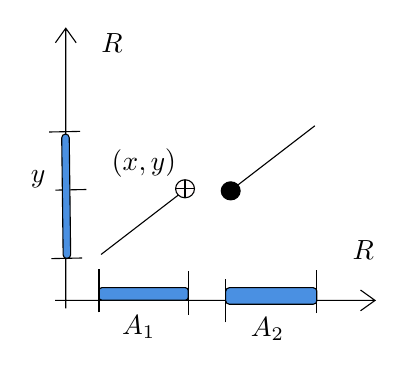
\begin{tikzpicture}[x=0.75pt,y=0.75pt,yscale=-1,xscale=1]
%uncomment if require: \path (0,300); %set diagram left start at 0, and has height of 300

%Shape: Axis 2D [id:dp26430596329710565] 
\draw  (49,214.44) -- (203.1,214.44)(54.1,83.3) -- (54.1,218.3) (196.1,209.44) -- (203.1,214.44) -- (196.1,219.44) (49.1,90.3) -- (54.1,83.3) -- (59.1,90.3)  ;
%Rounded Rect [id:dp051838128654554616] 
\draw  [fill={rgb, 255:red, 74; green, 144; blue, 226 }  ,fill opacity=1 ] (70.1,209.67) .. controls (70.1,208.91) and (70.71,208.3) .. (71.47,208.3) -- (111.74,208.3) .. controls (112.49,208.3) and (113.1,208.91) .. (113.1,209.67) -- (113.1,212.94) .. controls (113.1,213.69) and (112.49,214.3) .. (111.74,214.3) -- (71.47,214.3) .. controls (70.71,214.3) and (70.1,213.69) .. (70.1,212.94) -- cycle ;
%Rounded Rect [id:dp4090774294526508] 
\draw  [fill={rgb, 255:red, 74; green, 144; blue, 226 }  ,fill opacity=1 ] (131.1,210.12) .. controls (131.1,209.11) and (131.91,208.3) .. (132.92,208.3) -- (173.28,208.3) .. controls (174.29,208.3) and (175.1,209.11) .. (175.1,210.12) -- (175.1,214.48) .. controls (175.1,215.49) and (174.29,216.3) .. (173.28,216.3) -- (132.92,216.3) .. controls (131.91,216.3) and (131.1,215.49) .. (131.1,214.48) -- cycle ;
%Straight Lines [id:da64388132407526] 
\draw    (110.1,162.3) -- (71.1,192.3) ;
\draw  [fill={rgb, 255:red, 255; green, 250; blue, 250 }  ,fill opacity=1 ] (107,160.65) .. controls (107,158.25) and (109.04,156.3) .. (111.55,156.3) .. controls (114.06,156.3) and (116.1,158.25) .. (116.1,160.65) .. controls (116.1,163.05) and (114.06,165) .. (111.55,165) .. controls (109.04,165) and (107,163.05) .. (107,160.65) -- cycle ; \draw   (107,160.65) -- (116.1,160.65) ; \draw   (111.55,156.3) -- (111.55,165) ;
\draw  [fill={rgb, 255:red, 0; green, 0; blue, 0 }  ,fill opacity=1 ] (129,161.65) .. controls (129,159.25) and (131.04,157.3) .. (133.55,157.3) .. controls (136.06,157.3) and (138.1,159.25) .. (138.1,161.65) .. controls (138.1,164.05) and (136.06,166) .. (133.55,166) .. controls (131.04,166) and (129,164.05) .. (129,161.65) -- cycle ; \draw   (129,161.65) -- (138.1,161.65) ; \draw   (133.55,157.3) -- (133.55,166) ;
%Straight Lines [id:da6240534914484722] 
\draw    (174.1,130.3) -- (135.1,160.3) ;
%Straight Lines [id:da26345564387084763] 
\draw    (64,161) -- (49.1,161.3) ;
%Rounded Rect [id:dp5446725714009876] 
\draw  [fill={rgb, 255:red, 74; green, 144; blue, 226 }  ,fill opacity=1 ] (54.66,194.29) .. controls (53.66,194.31) and (52.84,193.5) .. (52.82,192.5) -- (52.13,136.12) .. controls (52.12,135.12) and (52.92,134.3) .. (53.92,134.29) -- (53.92,134.29) .. controls (54.92,134.28) and (55.74,135.08) .. (55.76,136.08) -- (56.44,192.46) .. controls (56.46,193.46) and (55.66,194.28) .. (54.66,194.29) -- cycle ;
%Straight Lines [id:da09701668858062606] 
\draw    (113.1,221.3) -- (113.1,200.3) ;
%Straight Lines [id:da006128268425505956] 
\draw    (70.1,220.17) -- (70.1,199.17) ;
%Straight Lines [id:da2642800457448089] 
\draw    (175.1,220.62) -- (175.1,199.62) ;
%Straight Lines [id:da346987503804841] 
\draw    (131.1,224.98) -- (131.1,203.98) ;
%Straight Lines [id:da3019826841878914] 
\draw    (61,133) -- (46.1,133.3) ;
%Straight Lines [id:da641826860041459] 
\draw    (62,194) -- (47.1,194.3) ;

% Text Node
\draw (80,220.4) node [anchor=north west][inner sep=0.75pt]    {$A_{1}$};
% Text Node
\draw (142,221.4) node [anchor=north west][inner sep=0.75pt]    {$A_{2}$};
% Text Node
\draw (70,84.4) node [anchor=north west][inner sep=0.75pt]    {$\mathbb{R}$};
% Text Node
\draw (191,184.4) node [anchor=north west][inner sep=0.75pt]    {$\mathbb{R}$};
% Text Node
\draw (74.85,140.59) node [anchor=north west][inner sep=0.75pt]  [rotate=-359.42,xslant=-0.01]  {$( x,y)$};
% Text Node
\draw (36,150.4) node [anchor=north west][inner sep=0.75pt]    {$y$};


\end{tikzpicture}

\begin{exercice}
    Quelle est la topologie induite sur $\mathcal C$ le tryadique de Cantor ?
\end{exercice}

\begin{proposition}
    Soient $(X,\topologie_X)$ et $(Y,\topologie_Y)$ deux espaces topologique. $F:X\to Y$ est continue en $a\in \dom F$ si 
    \[
    \forall W \text{ voisinage pour } \topologie_Y \text{ de } F(a), \exists V  \text{ voisinage pour } \topologie_X \text{ de } a \text{ tel que } F(V)\subseteq W
    \]
    Cela est équivalent à
    \[
    \forall \ouvert \in \topologie_Y F(a)\in \ouvert, \exists \ouvert '\in \topologie_X, a \in \ouvert' \text{ tel que } F(\ouvert')\subseteq \ouvert
    \]
\end{proposition}

\begin{proof}
    Je l'ai faite dans ma tête, wallah c'est facile.
\end{proof}

\section{Topologie produit}
\subsection{Fonctions projections}
Soit $(X_i,\topologie_i)_{i\in I}$ une famille d'espaces $X\ne\varnothing$. On voudrait construire une topologie sur $\prod_{i\in I}X_i\ne\varnothing$. 
Les bébés considèrent les fonctions de projection $p_{i_0} : \prod_{i\in I}X_i\to X_{i_0}$. La topologie produit est la topologie la plus gorssière sur $\prod_{i\in I}X_i$ qui rend toutes les projections continues? 
\begin{definition}
    Sur un espace $X$, on dit que $\topologie_1$ est plus grossière  que $\topologie_2$ ou que $\topologie_2$ est plus fine que $\topologie_1$ si $\topologie_1\subseteq \topologie_2\subseteq\partie X$
\end{definition}
\begin{definition}
Soit $f$ une fonction entre deux ensembles munis d'une distance.
    $f$ est lipschitzien de constante $k\ge 0$ sur $I$ si $\forall x,y\in I$ $$d_{\im f}(f(x),f(y))\le k d_{\dom f}(x,y)$$
\end{definition}
\begin{definition}[Rappel]
    Soit $f:(X,\topologie_X)\to(Y,\topologie_Y)$. $f$ est continue si pour tout ouvert $\ouvert\in\topologie_Y$, $f^{-1}(\ouvert)\in\topologie_X$. Si $\topologie_Y$ admet une base $B$, on peut se limiter aux ouverts de la base, car tout ouvert de $\topologie_Y$ est une union d'ouverts de base. 
\end{definition}
On veut donc que $\topologie_{\prod X_i}$comprennent $P_{i_0}^{-1}(\ouvert)$ où $\ouvert \in \topologie_{i_0}$
$$\topologie_{\prod X_i} = \{p_{i_O}^{-1}\mid \ouvert\in\topologie_{i_0}\land i_0\in I\} = \{(\prod_{i\ne i_0}X_i)\times \ouvert\}$$

\begin{exercice}
    Une fonction continue sur son domaine (en tout point) ssi $\forall \ouvert$ de $\im f$ $f^{-1}(\ouvert)$ ouvert de $\dom f$
\end{exercice}

\begin{remarque}
On a $P_1^{-1}(\ouvert ) \cap P_2^{-1}(\ouvert)\neq \varnothing$ 
\end{remarque}

C'est en fait, on obtient la topologie usuelle. En effet, une base de la topologie produit est fournie par
\[
\{P_{i_1}^{-1}(\ouvert_{i_1})\cap P_{i_k}^{-1}(\ouvert _{i_k}) \mid  i_{1,\dotsc,k}\in I, \: \ouvert_{i_j}\in \topologie_{i_j}\}
\]
\begin{remarque}
    $(X,\topologie)$ et $Y$ en bijection avec $X$. Comment définir une topologie $\topologie_Y$ sur $Y$ qui copie celle de $X$ ? telle que ces deux espaces soient homéomorphes c'est à dire, il eciste une bijection bicontinue entre $X$ et $Y$. Par hypothèse, on a $F$ bijection de $X\to  Y$, on veut construire $\topologie_Y$ de telle sorte quue $F$ et $F^{-1}$ sont continues.
    Je veux que $F$ soit d'abord continue, c'est à dire que $\forall \ouvert \in \topologie_X$, il faut $F^{-1}(\ouvert)\in \topologie$ Pour $\topologie_Y$, on prend la topologie engendrée par les $F^{-1}(\ouvert)$ tel que $\ouvert \in \topologie_X$. De plus, $F^{-1}(\ouvert _1)\cap F^{-1}(\ouvert_2)= F^{-1}(\ouvert_1\cap \ouvert_2)$
 \end{remarque}

 \subsection{Lien avec triadique de Cantor}

 On sait que $\mathscr C \simeq 2^{\N}$ Une suite est une branche d'arbre binaire. Il faut choisir la topologie qu'on met sur $2^\N$ (il y en a $4$). On choisit la topologie discrète sur chaque fibre. Ainsi la topologie produit qui est l'union finie des segments initiaux. (C'est la même ttopologie sur les algèbres de bool) Cette topologie est compact. Voyons ce que cela signifie.

 



 \section{Densité}

 \subsection{Caractérisation}
Soit $(X,\topologie)$ un espace topologique, on dit que $Y$ est ($\topologie-$)dense dans $X$ si pour tout $\ouvert\in \topologie,\ \ouvert\cap Y\neq \varnothing$,  (ce qui est équivalent, en acceptant l'axiome du choix, à  pour tout $\ouvert\in\topologie$, il existe $y_o\in \ouvert\cap Y$). De façon équivalente, on peut dire $Y$ est dense dans $X$ ssi pour tout voisinage $V$, il existe $y\in V\cap Y$.Si $\topologie$ admet une base $S$ alors c'est équivalent à ce que $\forall B\in S,\ B\cap Y\ne\varnothing$. 
\begin{exemple}
    $\mathbb{Q}$ est $\topologie_2-$dense dans $\R$. On utilise le fait que tout ouvert est une union de boules ouvertes; donc  il suffit de prouver que si
    $B(x,r)$ est une boule ouverte, j'y trouve un rationnel. Ici $B(x,r)=]x-r,x+r[$, il faut trouver $q\in ]x-r,x+r[$ Comment placer un rationnel $r-$proche de $x$ ? Si on admet que les réels sont des limites de suites de Cauchy de rationnels, on prend une telle suite $q_n$ convergeant vers $x$ et on sait qu'il existe $n_0$ tel que pour tout $n\geq n_0\quad |q_n-x|\leq \frac{r}{2}$
   Considérons l'écriture décimale de $x$, càd prenons $z\in\Z,\forall i\in\N_0, d_i\in\{0,1,\ldots,9\}$ tels que $x=\overline{ z,d_1d_2...d_k...}_{10}$ ou autrement dit $x=z+\sum_{i=1}^\infty d_i10^{-i}$
    Et clairement $x_k=z+\sum_{i=1}^kd_i10^{-i}$ vérifie que 
    \[
    |x-x_k|=\sum_{i=k+1}^\infty d_i10^{-i}\leq g\sum_{i=k+1}^\infty10^{-i}=g\cdot10^{-(k+1)}\sum_{i=0}^\infty10^{-i}=g\cdot10^{-(k+1)}\frac{1}{1-\frac{1}{10}}=10^{-k}
    \]
    On cherche $q\in ]x-r,x+r[$. On peut pour cela prendre $x_k$ tel que $|x-x_k|\leq \frac{r}{2}$ càd tel que $10^{-k}\leq \frac{r}{2}$.
\end{exemple}
\begin{remarque}
    Tout cela est possible car $\R$ est un groupe archimédien (dont l'ordre est en plus compatible avec $\cdot$)
    \[
    \R^{\geq0}=\bigsqcup_{n\in \N}[n,n+1[
    \]
\end{remarque}
\begin{definition}
    Un groupe ordonné $(G,+,\leq)$ est dit archimédien si $\leq$ est total, compatible avec plus et tel que $\forall a\in G^{>0},\forall b\in G^{\geq 0},\ \exists n\in\N, an\geq b$
\end{definition}


\begin{proposition}
        Soit une boule ouverte $B(x,r)$ non vide de $\R^2$, alors $B(x,r)\cap \Q^2\neq \emptyset$. 
\end{proposition}

\begin{proof}
on a que $x=(x_1,x_2)$ où $x_1,x_2\in \R$. Par définition de $\R$. Il existe $(q_{1_n})_{n\in I}\subseteq \Q$ et $(q_{2_n})_{ n\in J }\subseteq \Q$ convergeant respectivement vers $x_1$ et $x_2$. On considère donc la suite $(q_n)_{n\in I\cap J}\subseteq \Q^2$ où $q_n=(q_{1_n},q_{2_n})$. Puisque la convergence des suites dans $\R^n$ revient à la convergence coordonnée par coordonnée. On a donc trouvé une suite $(q_n)\subseteq \Q^2$ convergeant vers $x\in\R$. Nous avons donc :
\begin{equation*}
    \forall\varepsilon>0, \exists n_0\in I\cap J, \forall n\geq n_0 \quad \norm{q_n-x}<\varepsilon
\end{equation*}
On utilise l'équation avec $\varepsilon=r$, il existe donc $n_0\in I\cap J$ tel que $\norm{q_{n_0}-x}< r$. On a donc $q_{n_0}\in B(x,r)\cap \Q^2$. Autrement dit, on vient de montrer que 
\[
B(x,r)\cap \Q^2\neq \varnothing
\]
\end{proof}

Avec ce résultat, prouvons que l'intersection de $2$ boules ouvertes de $\R^2$ est une union dénombrable de boules ouvertes.
\[
B_1\cap B_2\neq \emptyset
\]
On considère
$\mathbb{Q}^2\cap (B_1\cap B_2)\neq \emptyset$
En fait, il existe $S$ dénombrable tel que $\topologie_2=(S)$. \begin{proposition}
    Toute $B(x,r)$ est une union dénombrable de $B\left(x, \frac{1}{n}\right)$ avec $x\in \mathbb{Q}^2 $
\end{proposition}
\begin{proof}
    Montrons que $B(x,r)= \bigcup_{(q,\varepsilon)\in Q}B(q,\varepsilon)$ avec $Q:=\{(q,\varepsilon)\in\Q^2\times \Q\mid \exists n\in\N,\ \varepsilon=\frac 1 n ,\ B(q,\varepsilon)\subseteq B(x,r)\}$.
    \begin{description}
        \item[$\supseteq$ : ]Trivial car tous les éléments de l'union sont $\subseteq B(x,r)$
        \item[$\subseteq$ : ]Soit $y\in B(x,r)$. Comme $r':= r-d(y,x)>0$, il existe par le point précédent $q_y\in \Q^2,\varepsilon_y\in\{\frac 1 n\mid n\in\N\}$ tels que $B(q_y,\varepsilon_y)\subseteq B(y,r')$. Soit $z\in B(y,r')$. On a $d(z,r)\leq d(y,z)+d(y,x)<r-d(y,x)+d(y,x) = r$ d'où $B(q_y,\varepsilon_y)\subseteq B(y,r')\subseteq B(x,r)$ et donc $y\in B(q_y,\varepsilon_y)\subseteq \bigcup_{(q,\varepsilon)\in Q}B(q,\varepsilon)$
    \end{description}
\end{proof}

\subsection{Prolongement des applications}

\section{Compacité}
\subsection{Définition et propriétés topologiques}

\subsection{compacité dans les espaces métriques}
 \begin{definition}
      Un espace métrique $(X,d)$ est complet ssi toute suite de Cauchy d'éléments de $X$ converge dans $X$.
  \end{definition}
  \begin{remarque}
      Considérons $\Q$ muni de la topologie induite par la topologie usuelle sur $\R$. Condidérons $\interoo{-\sqrt 2, -\sqrt 2}\cap \Q = \interff{-\sqrt 2, -\sqrt 2}\cap \Q $
  \end{remarque}
  Soit $X$ complet. Considérons $\ferme$ fermé. Alors $\ferme$ est compact pour la topologie induite.

 \begin{definition}
     Une topologie $\topologie$ est dite $T_2$ sur l'espace $X$, si $\forall x_1,x_2 \in X_1, \exists \ouvert_1 \text{ qui comprend }x_1 \exists \ouvert_2 \text{qui comprend }x_2 $, tel que $\ouvert_1\cap\ouvert_2\neq \varnothing$  
 \end{definition}
\begin{definition}
    On dit que $(X,\topologie)$ est précompact si toute famille de fermés de $\topologie$. qui à la \textit{P.I.F} à une intersection non vide. \textit{i.e} $\bigcap_{i\in I}F_i\neq \varnothing$
\end{definition}

\begin{exercice}
    Soit $I$ un ensemble non vide, soit $A\subseteq \partie (I)$ tel que $A$ à la pif. c'est à dire que $\forall x_1,\dotsc x_k\in A$ $\bigcap_{i=1}^kx_i\neq \varnothing$ alors $\langle A\rangle  = \{U\subseteq I \mid \text{une intersection finie d'élements de }A \subseteq U\}$
\end{exercice}

\begin{exercice}
    Un espace $(X,\topologie)$ est précompact si pour toute famille $(\ouvert_i)_{i\in I}$ d'ouvert de $\topologie$ qui recouvre $X$, il existe $I_0\subseteq I$ fini tel que $\cup \ouvert_i =X$. Autrement dit, de toute recouvrementt ouvert de $X$, on peut extraire un sous-recouvrement fini de $X$.
\end{exercice}
\begin{lemme}
    Soit $(\ferme_i)$ un famille de fermés de $X$. Soit $(\ferme^c_i)$ la famille d'ouverts associés. Supposons que $(\ferme_i)$ aient la PIF
\end{lemme}
\begin{remarque}
    $(F_i^c)$ est un recouvrement de $X$ ssi $\bigcup\ferme_i^c = X$ ssi $\bigcap \ferme_i = \varnothing$
\end{remarque}
\begin{remarque}
    $(\ferme_i)_{i\in I}$ a la pif ssi $$\forall  I_0\subseteq I, \text{ si $I_0$ est fini alors }\bigcap_{i\in I_0}\ferme_i\ne\varnothing$$ ssi $\bigcup_{i\in I_0}\ferme_i^c\ne X$
\end{remarque}
Par conséquent, chaque fois que j'ai une famille d'ouverts dont toutes les unions finies ne sont pas des recouvrement, alor la famille globale n'est pas un recouvrement. Donc, si j'ai (1), on a (1') et donc on a saussi la contraposée de (1') ui nous dit que si j'ai un recouvrement, alors il y avait un recouvrement fini de $X$. 
\begin{definition}
    Un espace $(X,\topologie)$ est dit compact s'il est précompact et $T_2$.
\end{definition}
 \begin{exemple}
     Soit $X$ avec la topologie discrète . $X$ est précompact ssi $X$ est fini.
 \end{exemple}
 \begin{proof}
     Les singletons sont ouverts.
 \end{proof}
 \begin{exemple}
     Considérons $\N\cup\{\omega\}$ muni de la topologie discrète sur $\N$ avec $\voisinage_\omega$ le filtre des cofinis sur $\N\cup\{\omega\}$. C'est le compactifié de $(\N,\topologie_\text{disc}$. Montrons que c'est un compact.
 \end{exemple}
 \begin{proof}
     Un recouvrement ouvert de $\N\cup\{\omega\}$ doit contenir $\omega$ donc prenons un cofini. Il ne reste qu'un nombre fini de points, donc ils peuvent être recouvert par un nombre fini d'ouverts. De plus cette topologie est $T_2$.
 \end{proof}
 \begin{definition}
     $X$ un espace métrique est dit séquentiellement compact ssi toute suite possède une sous-suite convergente.
 \end{definition}
 \begin{exercice}
     Soit $X$ un espace métrique. Montrer que $X$ est séquentiellement compact ssi il est précompact.
 \end{exercice}
 \begin{definition}
     Soit $(X,\topologie)$ un espace topologique. On dit que $K\subseteq X$ est (pré)compact ssi $K$ muni de la topologie induite par $\topologie$ est (pré)compact.
 \end{definition}
 \begin{proposition}
     L'image d'un compact $K$ par une fonction continue est un compact. 
 \end{proposition}
 \begin{proof}
     Soit $(\ouvert_i)$ une famille d'ouverts recouvrant $F(K)$. Alors la famille $(F^{-1}(\ouvert_i))$ est une famille d'ouverts
 \end{proof}

 \begin{proposition}
     Soit $(X,d)$ séquentiellement compact. Soit $Y$ muni d'un ordre. Soit $f : X\to Y$ une application continue. Alors si $a\in Y$ est la borne supérieure de $\im f$, alors $a\in\im f$.  
 \end{proposition}
 \begin{proof}
     Donc, on utilise le fait que l'image d'un précompact et compact
 \end{proof}

\begin{theoreme}[Tychonoff]
      Le produit d'espaces compacts d'une famille $(X_i,\topologie_i)_{i\in I}$, \textit{i.e.} $\prod_{i\in I}X_i$ muni de la topologie produit, est compact. 
  \end{theoreme}

 \section{Connexité}
\subsection{Définition et propriétés}
 \begin{definition}
     Un espace topologique $(X\topologie)$ est connexe ssi les seuls ouverts fermés de $X$ sont $\varnothing$ et $X$.
 \end{definition}

\begin{exercice}
    Montrer que $\R$ est connexes.
\end{exercice}

\begin{remarque}
    Vu nos constructions sur $(\Z, d_p)$ clairement $\Z$ n'est pas connexe.
\end{remarque}

 \subsection{Composantes connexes}

 % ----------------------------------------------------------------

\begin{lemme}
Soit $(X, \mathcal{T})$ un espace topologique et $A, B$ des sous-ensembles.
Si $A$ et $B$ sont tous les deux connexes (pour la topologie induite) et $A \cap B$
est non-vide, alors $A \cup B$ est connexe (pour la topologie induite).
\end{lemme}

\begin{proof}
Supposons que $A \cup B$ ne soit pas connexe. Il existe alors une partition
$A \cup B = U \sqcup V$ avec $U, V$ ouverts non vides dans la topologie induite
sur $A \cup B$.

Considérons la restriction à $A$ : $A = (U \cap A) \sqcup (V \cap A)$. Comme $A$
est connexe, l'un des deux est vide, disons $V \cap A = \emptyset$, donc $A \subseteq U$.
De même, $B$ étant connexe, on obtient soit $B \subseteq U$, soit $B \subseteq V$.

Si $B \subseteq V$, alors $A \cap B \subseteq U \cap V = \emptyset$, ce qui contredit
$A \cap B \neq \emptyset$. Donc $B \subseteq U$, et ainsi $A \cup B \subseteq U$,
ce qui contredit $V \neq \emptyset$. \qed
\end{proof}

% ----------------------------------------------------------------

\begin{lemme}
Soit $(X, \mathcal{T})$ un espace topologique, $E$ un sous-ensemble de $X$ muni
de la topologie induite par $\mathcal{T}$, notée dans cet énoncé $\mathcal{T}_E$.
Soit $A \subseteq E$, muni de la topologie induite par $\mathcal{T}_E$. Alors cette
topologie induite est la même que celle induite par $\mathcal{T}$ sur $A$ comme
sous-ensemble de $X$.
\end{lemme}

\begin{proof}
Un ouvert de la topologie induite par $\mathcal{T}_E$ sur $A$ est de la forme
$A \cap V$ où $V \in \mathcal{T}_E$, i.e.\ $V = E \cap U$ pour un certain $U \in \mathcal{T}$.
Donc $A \cap V = A \cap E \cap U = A \cap U$ (car $A \subseteq E$), qui est
bien un ouvert de la topologie induite par $\mathcal{T}$ sur $A$. La réciproque est
immédiate. \qed
\end{proof}

% ----------------------------------------------------------------

\begin{lemme}[Existence]
Soit $(X, \mathcal{T})$ un espace topologique, $E$ un sous-ensemble de $X$ et
$x \in E$. Il existe $A \subseteq X$ tel que :
\begin{itemize}
    \item $A \subseteq E$ ;
    \item $x \in A$ ;
    \item $A$ est connexe pour la topologie induite,
\end{itemize}
et $A$ est maximal pour l'inclusion.
\end{lemme}

\begin{proof}
Posons
\[
    A = \bigcup_{\substack{C \subseteq E,\, x \in C \\ C \text{ connexe}}} C.
\]
Cet ensemble contient $x$ (car $\{x\}$ est connexe) et est inclus dans $E$.
Il reste à montrer que $A$ est connexe. Soit $C_1, C_2$ deux ensembles connexes
de cette union tels que $C_1 \cap C_2 \ni x \neq \emptyset$. Par le Lemme,
$C_1 \cup C_2$ est connexe. Une union quelconque d'ensembles connexes partageant
tous le point $x$ est connexe par une récurrence transfinie (ou argument de Zorn),
donc $A$ est connexe. La maximalité découle directement de la définition de $A$
comme union de tous les connexes contenant $x$ dans $E$. \qed
\end{proof}

% ----------------------------------------------------------------

\begin{lemme}[Unicité]
Soit $(X, \mathcal{T})$ un espace topologique, $E$ un sous-ensemble de $X$ et
$x \in E$. Soient $A, B \subseteq X$ tels que :
\begin{itemize}
    \item $A, B \subseteq E$ ;
    \item $x \in A$ et $x \in B$ ;
    \item $A$ et $B$ sont connexes pour la topologie induite,
\end{itemize}
et $A$ et $B$ sont maximaux pour l'inclusion. On a que $A = B$.
\end{lemme}

\begin{proof}
Puisque $x \in A \cap B$, on a $A \cap B \neq \emptyset$. Par le Lemme~9,
$A \cup B$ est connexe, $A \cup B \subseteq E$, et $x \in A \cup B$.
Par maximalité de $A$, on a $A \cup B \subseteq A$, donc $B \subseteq A$.
Par maximalité de $B$, de même $A \subseteq B$. Ainsi $A = B$. \qed
\end{proof}

% ----------------------------------------------------------------

\begin{definition}[Composante connexe]
Soit $(X, \mathcal{T})$ un espace topologique, $E$ un sous-ensemble de $X$ et
$x \in E$. La \textbf{composante connexe} de $x$, relativement à $E$, notée $C_x$,
est l'ensemble connexe maximal contenant $x$ et inclus dans $E$.

\medskip
L'existence et l'unicité de la composante connexe sont données par les deux
lemmes précédents.
\end{definition}

\medskip
Dans ce qui suit, quand le contexte est clair, nous n'ajoutons pas la précision
« relativement à $E$ ».

% ----------------------------------------------------------------

\begin{lemme}
Soit $(X, \mathcal{T})$ un espace topologique, $E$ un sous-ensemble de $X$ et
$x, y \in E$. Si $x \in C_y$ alors $C_x = C_y$.
\end{lemme}

\begin{proof}
Si $x \in C_y$, alors $C_x \cap C_y \ni x \neq \emptyset$. Par le Lemme~9,
$C_x \cup C_y$ est connexe, contient $y$, et est inclus dans $E$. Par maximalité
de $C_y$, on a $C_x \cup C_y \subseteq C_y$, donc $C_x \subseteq C_y$. Par
maximalité de $C_x$, on a $C_y \subseteq C_x$. Donc $C_x = C_y$. \qed
\end{proof}

% ----------------------------------------------------------------

\begin{lemme}
Soit $(X, \mathcal{T})$ un espace topologique, $E$ un sous-ensemble de $X$ et
$x, y \in E$. Si $x \notin C_y$ alors $C_x \cap C_y = \emptyset$.
\end{lemme}

\begin{proof}
Supposons $C_x \cap C_y \neq \emptyset$. Par le Lemme~9, $C_x \cup C_y$ est
connexe, contient $y$, et est inclus dans $E$. Par maximalité de $C_y$,
$C_x \cup C_y \subseteq C_y$, donc $C_x \subseteq C_y$, d'où $x \in C_y$,
ce qui contredit l'hypothèse. \qed
\end{proof}

% ----------------------------------------------------------------

\begin{theoreme}[Partition]
Les composantes connexes des éléments d'un ensemble forment une partition de
cet ensemble.
\end{theoreme}

\begin{proof}
Soit $E$ un sous-ensemble de $(X, \mathcal{T})$. Pour tout $x \in E$, on a
$x \in C_x$ (car $\{x\}$ est connexe et inclus dans $E$), donc
$\displaystyle E = \bigcup_{x \in E} C_x$.

Il reste à montrer que deux composantes connexes sont soit égales, soit disjointes.
Soient $x, y \in E$. Soit $C_x \cap C_y \neq \emptyset$ : par le Lemme~16,
$x \in C_y$, et par le Lemme~16 aussi (en échangeant les rôles), $C_x = C_y$.
Soit $C_x \cap C_y = \emptyset$. Donc les composantes connexes forment bien une
partition de $E$. \qed
\end{proof}

